\documentclass[12pt,a4paper,onecolumn]{article}
\usepackage[utf8]{inputenc}
\usepackage[ngerman]{babel}
\usepackage{datetime}
\usepackage[autostyle]{csquotes}
\usepackage{hyperref}
\usepackage{graphicx}
\usepackage[toc]{glossaries}
\makeglossaries

\newcommand\titleofdoc{StayHealthy} % Put your document title in this argument
\newcommand\GroupName{Team 6} % Put your group name here. If you are the only member of the group, just put your name


\newglossaryentry{Trainingseinheit}
{
    name=Trainingseinheit,
    description={ist eine Sammlung von Übungen mit deren Menge in Wiederholungen
    bzw. Minuten}
}

\newglossaryentry{Trainingsplan}
{
    name=Trainingsplan,
    description={Ein Trainingsplan ist ein wöchentlicher Plan der aus einer oder mehreren, gleichen oder verschiedenen, Trainingseinheiten besteht}
}

\newglossaryentry{Mahlzeit}
{
    name=Mahlzeit,
    description={Eine Mahlzeit ist eine Sammlung von Speisen und deren Menge in Gramm.}
}

\newglossaryentry{Ernährungsplan}
{
    name=Ernährungsplan,
    description={Ein Ernährungsplan ist ein wöchentlicher Plan der aus ein oder mehreren Mahlzeiten besteht.}
}

\newglossaryentry{Zeitplan}
{
    name=Zeitplan,
    description={Ein Zeitplan besteht aus ein oder mehreren Ernährungsplänen, sowie aus ein oder mehreren Trainingsplänen}
}

\newglossaryentry{Sportler}
{
    name=Sportler,
    description={Ein Sportler ist ein Benutzer, welcher die Funktion der Software nutzt in Bezug auf die Nutzung des Trainings- bzw. Ernhährungsplans.}
}

\newglossaryentry{Übung}
{
    name=Übung,
    description={ist z.B. 1 Liegestütze oder 1 Minute Laufen}
}

\newglossaryentry{Speise}
{
    name=Speise,
    description={ist z.B. 1 Gramm Tomaten.}
}

\newglossaryentry{Personaltrainer}
{
    name=Personaltrainer,
    description={ist ein Benutzer.}
}

\begin{document}
\begin{titlepage}
   \begin{center}
        \vspace*{4cm} % Adjust spacings to ensure the title page is generally filled with text

        \Huge{\titleofdoc} 

        \vspace{0.5cm}
        \LARGE{Anforderungsspezifikation}
            
        \vspace{3 cm}
        \Large{\GroupName}
       
        \vspace{0.25cm}
        \large{Andreas Wirth, Marco Klein, Khader AlHamed, Denis Manherz}
       
        \vspace{3 cm}
        \Large{\today}% change date format to dd.mm.yyyy
        
        \vspace{0.25 cm}
        \Large{Software Praktikum}
       

       \vfill
    \end{center}
\end{titlepage}
\setcounter{page}{2}
\tableofcontents
\newpage

\section{Dokumentinformationen} 
\subsection{Änderungsgeschichte}
\begin{center}
\begin{tabular}{ |c|c|c|c| } 
 \hline
 Datum & Version & Änderung & Autor\\ 
 \hline
 25.03.2022 & 0.0 & Inhaltsverzeichnis & Denis Manherz \\ 
 \hline
 31.03.2022 & 1.0 & bis Abschnitt 5 & Denis Manherz \\ 
 \hline
 01.04.2022 & 1.1 & Use Cases Fully Dressed & Marco Klein \\ 
 \hline
 01.04.2022 & 1.2 & Use Cases Fully Dressed & Khader Alhamed \\ 
 \hline
\end{tabular}
\end{center}

\section{Einführung}
\subsection{Definitionen und Abkürzungen}
\textbf{Ernährungsverhalten} - Ernährungsbezogene Handlungen die Menschen im Alltag vollziehen\\
\textbf{Gesundheitsverhalten} - Handlungen von gesunden Menschen die das Risiko von Erkrankungen nachweislich senken oder welche die Gesundheit positiv beeinflussen.\\
\textbf{Kalorie} - 1 kcal\\
\textbf{Grundumsatz} - Anzahl der Kalorien die zur Aufrechterhaltung der Lebensfunktionen benötigt wird\\
\textbf{Trainingsart} - Ausdauer- oder Krafttraining
\subsection{Referenzen}
\href{https://sceweb.uhcl.edu/helm/RationalUnifiedProcess/webtmpl/templates/req/rup_srs.htm}{sceweb.uhcl.edu - Software Reqirements Specification}
\subsection{Übersicht}
Dieses Dokument bietet eine allgemeine Beschreibung der Software StayHealthy. Darüber hinaus werden nichtfunktionale sowie funktionale Anforderungen erläutert. Zum Schluss werden die Use Cases des Produkts im Fully Dressed Format dargestellt.

\section{Allgemeine Beschreibung}
\subsection{Produktperspektive}
Ein Lebensstil der sich positiv auf die allgemeine Gesundheit auswirkt und diese erhält wird für Menschen immer wichtiger. Die Software StayHealthy soll dem Endnutzer dabei helfen sein Ernährungsverhalten zu dokumentieren und ihm eine Übersicht darüber geben wie viel Sport er macht bzw. wieviele Kalorien er zu sich nimmt und verbraucht.\\ Mit den zugrundeliegenden Ernährungsdaten werden dem Benutzer mögliche sportliche Aktivitäten vorgeschlagen die ihm dabei helfen sollen einen gesunden Lebensstil zu pflegen. Natürlich kann der Benutzer auch selbstständig sportliche Aktivitäten dokumentieren. Darüber hinaus besteht die Möglichkeit sich von einem Personal Trainer Trainings- und Ernährungspläne erstellen zu lassen.
\subsection{Produktfunktion}
Die wesentliche Funktion von StayHealthy ist das dokumentieren von Kalorienaufnahme um anhand dieser körperliche Aktivitäten vorzuschlagen die den Kalorienhaushalt im Gleichgewicht halten.
Darüber hinaus werden dem Benutzer anhand von seinen angegebenen Präferenzen passende \gls{Mahlzeit}en vorgeschlagen.
\\Der Benutzer kann in der Anwendung \gls{Mahlzeit}en auswählen und angeben wie viel er von diesen zu sich genommen hat. Die Anwendung berechnet dann den Kaloriengehalt der angegebenen \gls{Mahlzeit}en. Außerdem gibt der Benutzer an, an welchen Tagen und zu welchen Tageszeiten er gerne trainieren möchte. 
\\Das System erstellt aus einer Auswahl von \gls{Übung}en einen Trainingplan für den jeweiligen Termin, hierbei werden natürlich auch die individuellen Benutzerdaten d.h. Kalorienaufnahme, Alter, Gewicht, Größe, Grundumsatz und Trainingsart berücksichtigt. Das System erinnert den Benutzer an bevorstehende \gls{Trainingseinheit}en. Der Benutzer kann diesen \gls{Trainingsplan} in seinem \gls{Zeitplan} bearbeiten, akzeptieren, ablehnen oder verschieben. \\Um dem Benutzer zu ermöglichen auch außerhalb seiner gewünschten Zeitslots zu trainieren, kann er einzelne \gls{Übung}en auswählen und die Zeit bzw. die Wiederholungen angeben. \\
Möchte der Benutzer gezielter trainieren kann er sein Profil upgraden. Dieses Upgrade ermöglicht es einem Personal Trainer Zugriff auf die Benutzerdaten zu bekommen und mit diesen je nach den Wünschen des Benutzers für diesen zugeschnittene Trainings- und Ernährungspläne zu erstellen.\\
Für einen Überblick wird dem Benutzer eine Statistik über sein Ernährungs- und Sportverhalten angeboten.\\
\newpage
\subsection{Benutzer Charakteristik}
Zielgruppe der StayHealthy Software sind Menschen die ihr Gesundheitsverhalten verbessern wollen aber noch nicht viel Erfahrung mit dem erstellen von \gls{Trainingseinheit}en haben bzw. noch nicht gezielt Sport gemacht haben.
\subsection{Einschränkungen}
Die Zusammenstellung der Trainingspläne geschieht nur anhand des Kalorienverbrauchs, der Trainingsart und den Präferenzen des Benutzers, andere Faktoren werden nicht berücksichtigt.
\\Es werden nur \gls{Übung}en angeboten die dem Prinzip des Bodyweight Trainings entsprechen, also dem Training mit dem eigenen Körpergewicht. Außerdem soll bei den \gls{Übung}en keine ausführliche Erklärung notwendig sein.\\
\subsection{Annahmen}
Die angegebenen Daten vom Benutzer sind richtig.

\section{Spezifische Anforderungen}
\subsection{Funktionale Anforderungen}
\subsubsection{Funktionale Anforderung - Benutzeraufwertung}
Das System markiert einen Benutzer als aufgewertet und ordnet diesen Benutzer einem Personal Trainer zu, der dann Zugriff auf die Benutzerdaten erhält.
\subsubsection{Funktionale Anforderung - Terminverwaltung}
Das System trägt Trainingspläne in den Kalender eines Benutzers ein, dabei berücksichtigt es die vom Benutzer präferierten Zeitslots.
\subsubsection{Funktionale Anforderung - Kalorienberechnung}
Das System berechnet den Kaloriengehalt der \gls{Mahlzeit}en und Ernährungspläne die der Benutzer erstellt hat und den Kalorienverbrauch von Trainingsplänen und Trainingseinheiten.
\subsubsection{Funktionale Anforderung - Grundumsatzberechnung}
Aus den Benutzerdaten berechnet das System den Grundumsatz des jeweiligen Benutzers.
\subsubsection{Funktionale Anforderung - Statistikerstellung}
Aus den gewonnenen Benutzerdaten erstellt das System eine Statistik über den Kalorienverbrauch und die sportliche Aktivität eines Benutzers über einen vom Benutzer gewählten Zeitraum in Tagen. Das heißt der Kalorienverbrauch wird mit der Kalorienaufnahme verglichen. Aufwärts- oder Abwertstrends für den Benutzer hervorgehoben.
\subsubsection{Funktionale Anforderung - Trainingsplanerstellung}
Je nach Kalorienaufnahme während er letzten 7 Tage eines Benutzers erstellt das System einen \gls{Trainingsplan} aus 3 Trainingseinheiten, die jeweils 3 verschiedene zufällige \gls{Übung}en enthalten, sodass Kalorienaufnahme, und Kalorienverbrauch im Gleichgewicht sind.
\subsubsection{Funktionale Anforderung - Erinnerung}
Das System erinnert den Benutzer einen Tag und nochmal eine Stunde vor Anfang einer \gls{Trainingseinheit}.

\subsection{Bedienbarkeit}
\subsubsection{Bedienbarkeitsanforderung - Benutzereingabe}
Die Bedienung der Software soll mit Maus und Tastatur erfolgen.
\subsubsection{Bedienbarkeitsanforderung - Übersichtlichkeit}
Über ein Menü wird es dem Benutzer ermöglicht alle Ansichten zu erreichen.
\subsubsection{Bedienbarkeitsanforderung - Benutzerfreundlichkeit}
Jede Ansicht soll dem Benutzer Funktionalitäten aus maximal einer Funktionalitätsgruppe zur Verfügung stellen, sowie sich auf einen Use Case beziehen.
\subsubsection{Bedienbarkeitsanforderung - Verständlichkeit}
Die Funktionen und Buttons sollen selbsterklärend sein, falls nötig wird eine Beschriftung hinzugefügt.

\subsection{Zuverlässigkeit}
\subsubsection{Zuverlässigkeitsanforderung - Datensicherheit}
Es soll sichergestellt werden das keine Benutzerdaten verloren gehen.
\subsection{Leistung}
\subsubsection{Leistungsanforderung - Antwortzeit}
Die Antwortzeit der Anwendung ist abhängig von der Datenbankzugriffszeit und der Zeit für Funktionalitätsberechnungen.
Die Berechnung von Funktionen soll maximal 20ms betragen.
\subsection{Wartbarkeit}
\subsubsection{Wartbarkeitsanforderung -Erweiterbarkeit}
Es soll sichergestellt werden, dass die Software jederzeit erweitert werden kann.
\subsection{Installation}
\subsubsection{Installationsanforderung - Windows}
Die Software ist mit Windows kompatibel und kann vorerst nur lokal auf dem System installiert und benutzt werden.
\subsection{Lokalisierung}
\subsubsection{Lokalisierungsanforderung}
Die StayHealthy Software soll zunächst auf dem nationalen Markt auf deutsch verfügbar sein.
\subsection{Schnittstellen}
\subsubsection{Benutzerschnittstellen}
Die Schnittstelle zum Benutzer erfolgt durch eine GUI.
\subsubsection{Softwareschnittstellen}
Die StayHealthy Software benötigt eine Schnittstelle zu einer Datenbank.
\subsubsection{Datenbankschnittstelle}
Die StayHealthy Software benötigt zur Speicherung seiner Daten eine Datenbank.
\subsection{Lizenzanforderungen}
Es werden keine Lizenzen benötigt die verwendete Datenbank ist eine kostenlose Version von Microsoft SQL Server.

\section{Use Cases}
\subsection{Use Case Diagram}
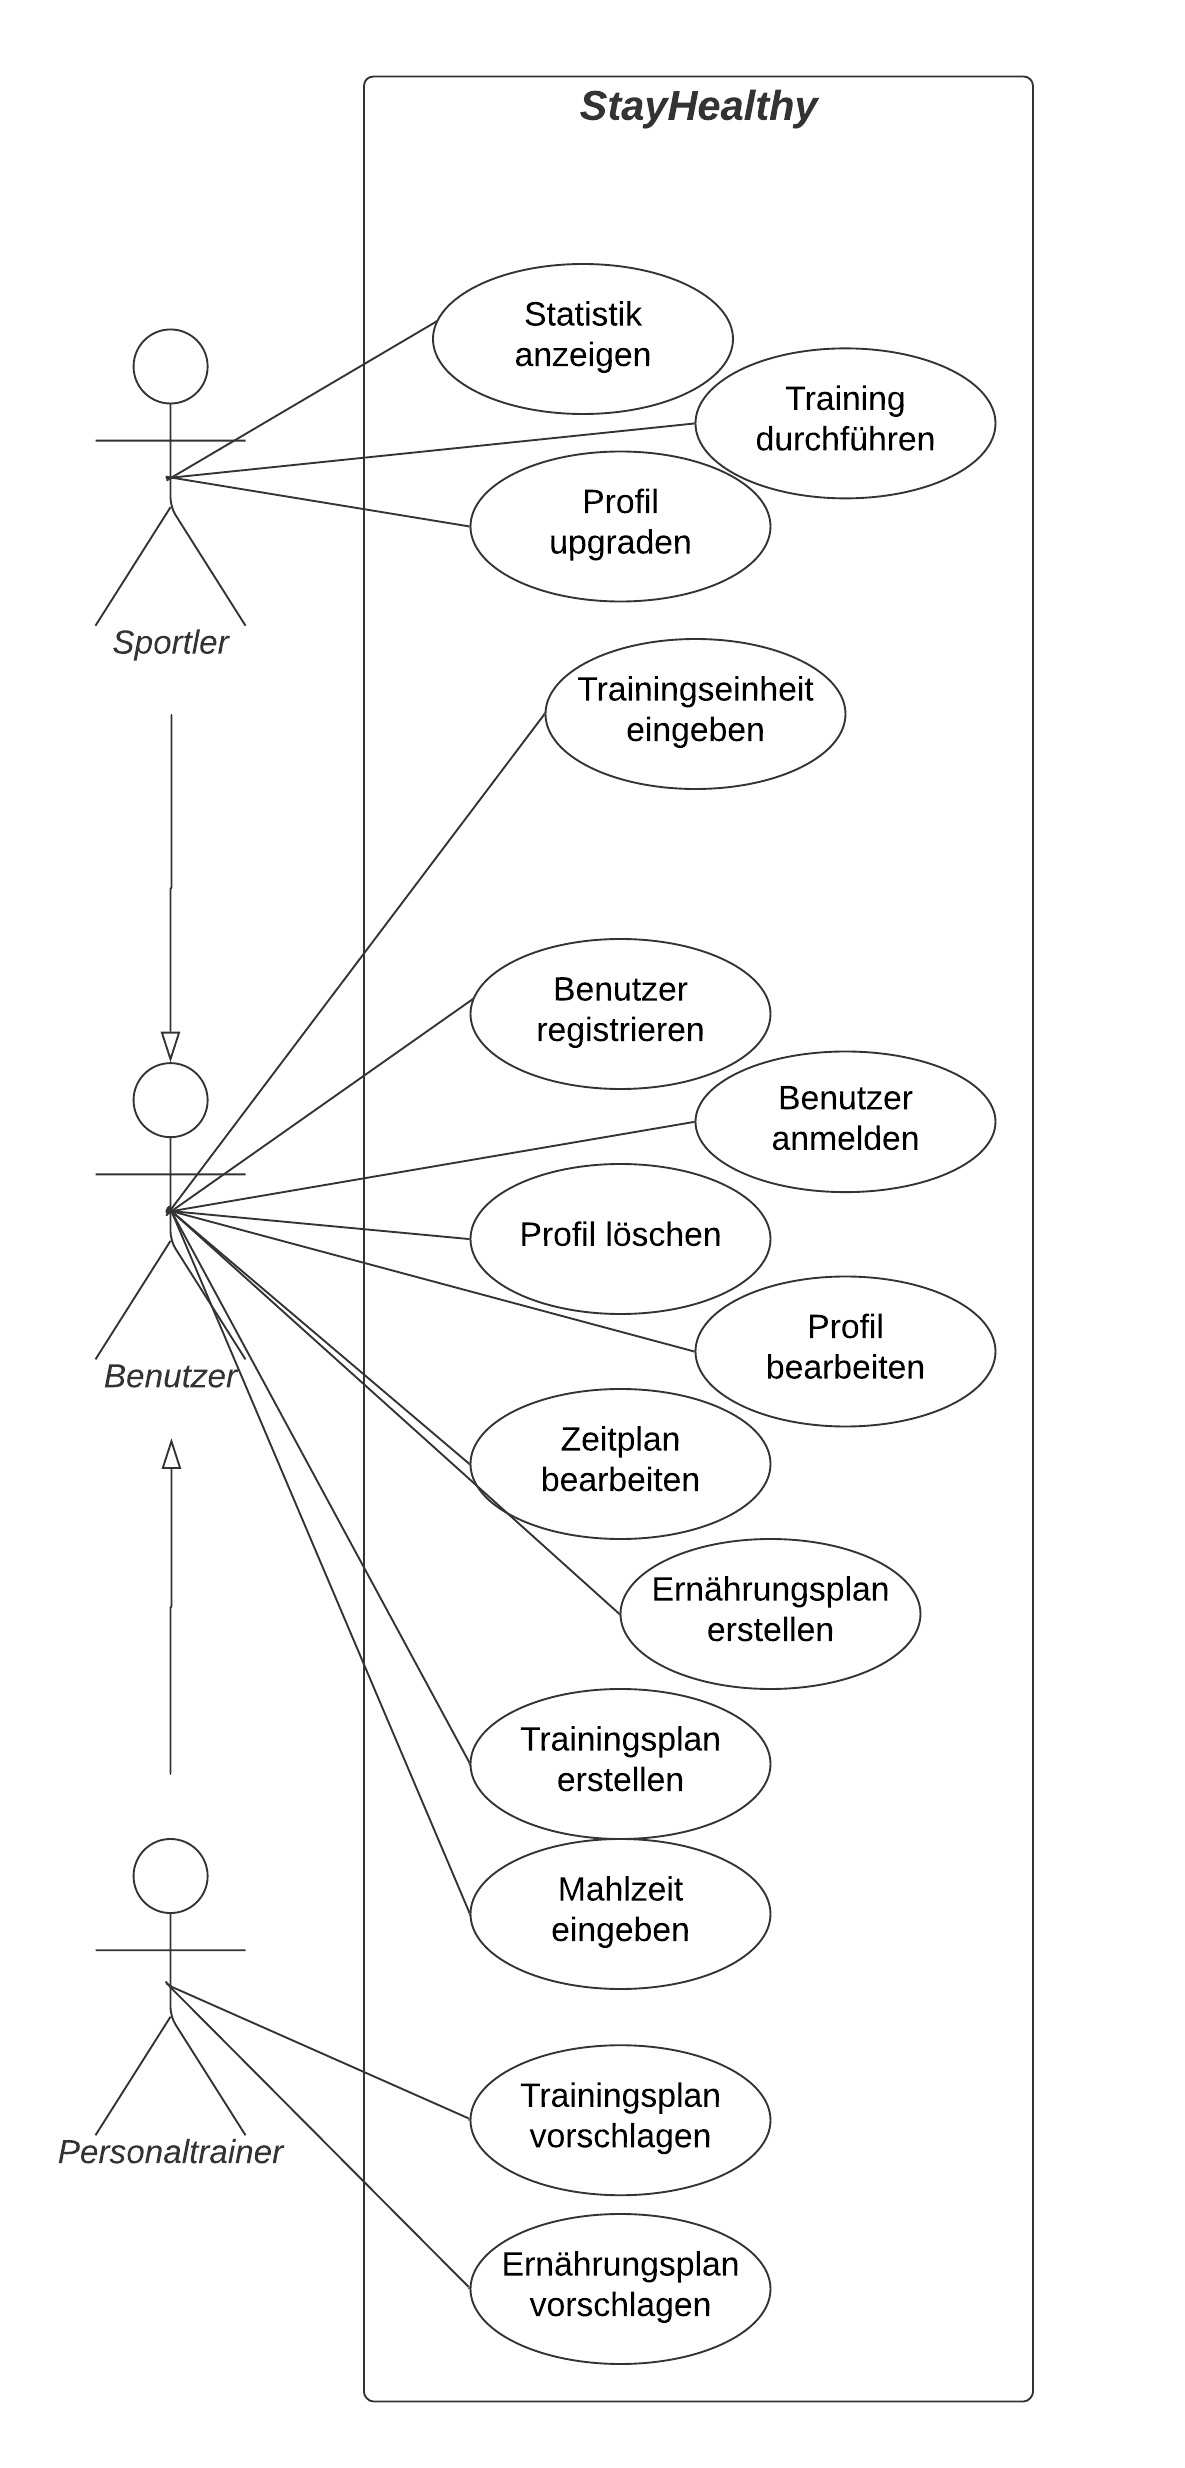
\includegraphics[scale=0.8]{Anwendungsfalldiagramm.png}

\subsection{Aktoren und Stakeholder}
Benutzer, Personal Trainer
\subsection{01 Use Case Benutzer registrieren}
\textbf{Primary Actor:}\\ Benutzer\\
\textbf{Stakeholders and Interests:}\\Benutzer will sich in der Anwendung registrieren.\\
\textbf{Preconditions:} \\Datenbank und Anwendung ist gestartet, der Benutzer befindet sich auf der Registrierungs Seite.\\
\textbf{Postconditions:}\\ Der Benutzer und seine Daten wurden erfolgreich in der Datenbank hinterlegt. \\
\textbf{Main Success Scenario:}
\begin{enumerate}
    \item System zeigt 'Anmelden' und 'Registrieren'
    \item Der Benutzer wählt Registrieren
    \item System fordert eine E-Mail Adresse
    \item Der Benutzer gibt einen E-Mail ein und bestätigt
    \item System fordert ein Passwort und Passwort wiederholen an
    \item Der Benutzer gibt einen Passwort und wiederholt und bestätigt es
    \item System gibt Hinweis 'erfolgreiche Registrierung'
    \item System zeigt wieder die zwei wähle 'anmelden','registrieren'
\end{enumerate}
\textbf{Extensions:}
\begin{enumerate}
    \item [4a.]  E-Mail ist schon in System vorhanden
    \begin{enumerate}
        \item[1.]System gibt Hinweis ' E-Mail bereits vorhanden ' und fordert erneut eine E-Mail Eingabe
        \item[2.]Benutzer macht weiter im MSS Schritt 4.
    \end{enumerate}
\end{enumerate}
\textbf{Frequency of Occurence:} \\Jeder Anwender kann sich mit einer E-Mail genau einmal registrieren\\

\subsection{02 Use Case Benutzer anmelden}
\textbf{Primary Actor:}\\ Benutzer\\
\textbf{Stakeholders and Interests:}\\
Benutzer will sich in der Anwendung anmelden.\\
\textbf{Preconditions:} \\ Der Benutzer hat sich registriert.\\
\textbf{Postconditions:}\\ Der Benutzer ist erfolgreich in der Anwendung angemeldet.\\
\textbf{Main Success Scenario:}
\begin{enumerate}
    \item Benutzer klickt den Button 'Anmelden'
    \item System fordert E-Mail und Passwort an
    \item Benutzer gibt seine E-Mail und Passwort und bestätigt 
    \item System gibt Hinweis „erfolgreiche Anmeldung“ 
    \item System Zeigt die Hauptmenü.
\end{enumerate}
\textbf{Extensions:}
\begin{enumerate}
    \item [3a.]  Der Benutzer macht eine ungültige Eingabe
    \begin{enumerate}
        \item[1.]System zeigt Hinweis 'falsche Benutzerdaten' und fordert erneute Eingabe
        \item[2.]Benutzer macht im MSS Schritt 2. weiter
    \end{enumerate}
\end{enumerate}
\textbf{Frequency of Occurence:}\\ Benutzer kann sich beliebig oft versuchen anzumelden.\\

\subsection{03 Use Case Profil Bearbeiten}
\textbf{Primary Actor:}\\ Benutzer\\
\textbf{Stakeholders and Interests:}\\
Benutzer seine Benutzerdaten ändern\\
\textbf{Preconditions:} \\ Datenbankserver ist gestartet. Der Benutzer befindet sich auf seiner Profilseite.\\
\textbf{Postconditions:}\\ Die aktualisierten Profildaten wurden in der Datenbank hinterlegt.\\
\textbf{Main Success Scenario:}
\begin{enumerate}
    \item Benutzer klickt den Button „Profil bearbeiten“
    \item System fordert Name, Nachname, Alter, Geschlecht , Größe, Übungspräferenz und Kalorien Aufnahme pro Woche an
    \item Benutzer gibt alle Daten ein und bestätigt
    \item System gibt ein Hinweis für die erfolgreiche Bearbeitung des Profils aus.
\end{enumerate}
\textbf{Extensions:}\\
\begin{enumerate}
    \item [3a.]Benutzer bestätigt die Eingabe nicht %braucht man das wenn der nutzer nicht bestätigt dann einfach keine änderung
    \begin{enumerate}
        \item [1.]System zeigt Auswahl "weiter bearbeiten"\\
        \item [2.]Benutzer wählt Auswahl und macht im MSS Schritt 3. weiter.\\
    \end{enumerate}
\end{enumerate} 
\textbf{Frequency of Occurence:}\\ beliebig oft pro Benutzer\\

\subsection{04 Use Case Profil löschen}
\textbf{Primary Actor:}\\ Benutzer\\
\textbf{Stakeholders and Interests:}\\
Benutzer will sein Profil löschen.\\
\textbf{Preconditions:} \\ Der Benutzer hat ein Profil erstellt und ist eingeloggt.\\
\textbf{Postconditions:}\\Der Benutzer hat sein Profil gelöscht.\\
\textbf{Main Success Scenario:}
\begin{enumerate}
    \item Benutzer klickt den Button 'Profil löschen'
    \item System fordert Benutzer auf sein Passwort einzugeben
    \item Benutzer gibt sein Passwort an
    \item System gibt Auswahl 'Profil löschen' und 'abbrechen'
    \item Benutzer bestätigt
    \item System bestätigt das Löschen
\end{enumerate}
\textbf{Extensions:}
\begin{enumerate}
    \item [3a.]  Benutzer gibt falsches Passwort
    \begin{enumerate}
        \item[1.]Weiter mit Schritt 2 des MSS
    \end{enumerate}
    \item [3b.]  Benutzer wählt 'abbrechen' aus
    \begin{enumerate}
        \item[1.]System zeigt das Hauptmenü
    \end{enumerate}
\end{enumerate}
\textbf{Frequency of Occurence:}\\ \\
Jedes Profil kann genau einmal gelöscht werden 

\subsection{05 Use Case Mahlzeit eingeben}
\textbf{Primary Actor:}\\ Benutzer\\
\textbf{Stakeholders and Interests:}\\
Benutzer will seine Mahlzeiten eingeben.\\
\textbf{Preconditions:} \\ Der Benutzer hat sich angemeldet.\\
\textbf{Postconditions:}\\Das System hat die vom Benutzer eingegebene \gls{Mahlzeit} in der Datenbank hinterlegt und
zeigt diese an.\\
\textbf{Main Success Scenario:}
\begin{enumerate}
    \item Benutzer klickt den Button 'Mahlzeit eingeben'
    \item System fordert Eingabe zu Anzahl die Speisen an
    \item Benutzer gibt die Anzahl ein
    \item System zeigt ein Tabelle mit Eingabe zu Beschreibung und Kalorien zu jeder Speise 
    \item Benutzer gibt die Daten ein
    \item System fordert Benutzer auf die Eingabe zu bestätigen oder Abbrechen
    \item Benutzer bestätigt
    \item System speichert die Eingabe in der Datenbank
\end{enumerate}
\textbf{Extensions:}
\begin{enumerate}
    \item [5a.]  Der Benutzer gibt nicht alle Daten ein
    \begin{enumerate}
        \item[1.] System zeigt einer Fehler Meldung und Weiter mit Schritt 4 des MSS
    \end{enumerate}
    \item [7a.]  Benutzer brecht ab\\
    \begin{enumerate}
        \item[1.]System zeigt die Hauptmenü
    \end{enumerate}
\end{enumerate}
\textbf{Frequency of Occurence:}\\ \\
Beliebig oft pro Benutzer. 

\subsection{06 Use Case Statistik anzeigen}
\textbf{Primary Actor:}\\ Benutzer\\
\textbf{Stakeholders and Interests:}\\
Benutzer will sich die Statistik von gesammelten Daten anzeigen lassen. \\
\textbf{Preconditions:} \\ Der Benutzer ist angemeldet und hat ein Profil erstellt. Benutzer hat mindestens eine \gls{Trainingseinheit} oder eine \gls{Mahlzeit} zu sich genommen. \\
\textbf{Postconditions:}\\Das System hat eine Statistik erstellt und zeigt diese dem Benutzer an.\\
\textbf{Main Success Scenario:}
\begin{enumerate}
    \item Benutzer klickt den Button 'Statistik anzeigen'
    \item System gibt Auswahl für einen Zeitraum zum Anzeigen der Statistik Tag,Woche,Monat
    \item Benutzer wählt Tag aus
    \item System zeigt ein Statistik mit Kalorie nehmen/verbrauchen für einen Tag
\end{enumerate}
\textbf{Extensions:}
\begin{enumerate}
    \item [3a.]  Benutzer wählt Woche oder Monat aus
    \begin{enumerate}
        \item[1.]System zeigt ein Statistik mit Kalorie nehmen/verbrauchen für einen Woche/Monat
    \end{enumerate}
\end{enumerate}
\textbf{Frequency of Occurence:}\\ \\
Beliebig oft pro Benutzer.

\subsection{07 Use Case Training durchführen}
\textbf{Primary Actor:}\\ Benutzer\\
\textbf{Stakeholders and Interests:}\\
Benutzer möchte die Durchführung einer \gls{Trainingseinheit} bestätigen.\\
\textbf{Preconditions:} \\  Der Benutzer hat sich angemeldet und ein Profil erstellt. Der Benutzer hat mindestens eine \gls{Trainingseinheit} im \gls{Trainingsplan} geplant. \\
\textbf{Postconditions:}\\Der Benutzer hat die Durchführung einer \gls{Trainingseinheit} bestätigt.\\
\textbf{Main Success Scenario:}
\begin{enumerate}
    \item Benutzer klickt den Button 'Training durchführen'
    \item System fordert eine Bestätigung ,dass der Benutzer jetzt mit seinem Training anfängt
    \item Benutzer bestätigt
    \item System zeigt den \gls{Trainingsplan} und zeigt eine Auswahl mit den \gls{Trainingseinheit}en, welche durchzuführen sind
    \item Benutzer erledigt Auswahl durch ankreuzen
    \item System fordert auf Eingabe zu bestätigen
    \item Benutzer bestätigt Eingabe
    \item System übernimmt die Daten der \gls{Trainingseinheit} in die Statistik
\end{enumerate}
\textbf{Extensions:}
\begin{enumerate}
    \item [6a.]  Benutzer bestätigt Eingabe nicht
    \begin{enumerate}
        \item[1.]System zeigt Auswahl 'Eingabe bearbeiten'
        \item[2.]Benutzer bestätigt Auswahl und macht im MSS Schritt 5. weiter
    \end{enumerate}
\end{enumerate}
\textbf{Frequency of Occurence:}\\ \\
Maximal so oft wie \gls{Trainingseinheit}en geplant wurden. 

\subsection{08 Use Case Training vorschlagen}
\textbf{Primary Actor:}\\ Benutzer\\
\textbf{Stakeholders and Interests:}\\
Benutzer will einen individuellen \gls{Trainingsplan} bekommen. \gls{Personaltrainer} erstellt einen individuellen \gls{Trainingsplan} für Benutzer.\\
\textbf{Preconditions:} \\ Der Benutzer hat sich angemeldet und ein Profil erstellt. Datenbankserver ist gestartet. Benutzer hat sein Profil geupgradet.\\
\textbf{Postconditions:}\\Der Benutzer hat einen individuellen \gls{Trainingsplan} bekommen.\\
\textbf{Main Success Scenario:}
\begin{enumerate}
    \item Benutzer klickt den Button „Personaltrainer“
    \item System zeigt Auswahl "Trainingsplan individuell erstellen"
    \item Benutzer bestätigt Auswahl
    \item System fordert für den Zeitraum von einer Woche für jeden Tag ein Datum und eine Uhrzeit an der trianiert werden will und ob trianiert werden will
    \item Benutzer macht die Eingabe der Daten
    \item System schlägt für jeden der Termine eine Traniningseinheit vor und fordert pro Vorschlag die Annahme des Vorschlages
    \item Benutzer bestätigt Vorschlag
    \item System übernimmt Vorschlag in den \gls{Trainingsplan} des \gls{Personaltrainer}es
    \item System fordert bei vollendeter Durchführung auf die Planung zu beenden mit 'beenden'
    \item Benutzer bestätigt mit 'beenden'
    \item System speichert \gls{Trainingsplan} und fügt diesen dem \gls{Zeitplan} hinzu
\end{enumerate} 
\textbf{Extensions:}\\
\begin{enumerate}
    \item [7a.]  Benutzer nimmt Vorschlag nicht an.
    \begin{enumerate}
        \item[1.]System fordert Benutzer auf selbst eine \gls{Trainingseinheit} zu wählen und zeigt Auswahl von der in Datenbank gespeicherteten \gls{Trainingseinheit}en.
        \item[2.]Benutzer wählt aus und bestätigt die Eingabe.
    \end{enumerate}
    \item [10a.] Benutzer bestätigt Eingabe nicht
     \begin{enumerate}
        \item[1.]System zeigt Auswahl 'Vorschläge überarbeiten'
        \item[2.]Benutzer wählt entsprechende Termine aus lehnt diese ab
        \item[3.]System fordert Benutzer auf selbst eine \gls{Trainingseinheit} zu wählen und zeigt Auswahl von der in Datenbank gespeicherten \gls{Trainingseinheit}en
        \item[4.]Benutzer wählt aus und bestätigt die Eingabe
    \end{enumerate}
\end{enumerate}
\textbf{Frequency of Occurence:}\\ \\
beliebig oft pro Benutzer

\subsection{09 Use Case Profil upgraden}
\textbf{Primary Actor:}\\ Benutzer\\
\textbf{Stakeholders and Interests:}\\
Benutzer möchte sein Profil upgraden um die Funktion des \gls{Personaltrainer}s zu nutzen.\\
\textbf{Preconditions:} \\ Benutzer hat ein Profil erstellt. 
Benutzer ist eingeloggt. Datenbankserver ist gestartet.\\
\textbf{Postconditions:}\\Benutzer hat ein Profil erfolgreich upgegradet.\\
\textbf{Main Success Scenario:}
\begin{enumerate}
    \item System zeigt Auswahl „Profil upgraden“.
    \item Benutzer wählt Auswahl „Profil upgraden“.
    \item System weist Benutzer einem \gls{Personaltrainer} zu.
\end{enumerate}
\textbf{Frequency of Occurence:}\\ \\
Einmal pro Benutzer.

\subsection{10 Use Case Zeitplan bearbeiten}
\textbf{Primary Actor:}\\ Benutzer\\
\textbf{Stakeholders and Interests:}\\
Benutzer möchte seinen \gls{Zeitplan} bearbeiten.\\
\textbf{Preconditions:} \\ Benutzer hat ein Profil erstellt. Benutzer ist eingeloggt. Datenbankserver ist gestartet.\\
\textbf{Postconditions:}\\Benutzer hat seinen \gls{Zeitplan} bearbeitet.\\
\textbf{Main Success Scenario:}
\begin{enumerate}
    \item Benutzer wählt die Option „Zeitplan bearbeiten“. 
    \item System gibt die Auswahl „bestehenden Termin ändern“.
    \item Benutzer gibt neue Trainingszeit ein.
    \item System fordert auf Eingabe zu bestätigen mit "bestätigen"
    \item Benutzer bestätigt
    \item System zeigt bearbeiteten \gls{Zeitplan} an
\end{enumerate}
\textbf{Extensions:}
\begin{enumerate}
    \item [1a.]  Benutzer wählt Auswahl „Plan löschen“
    \begin{enumerate}
        \item[1.]System zeigt Auswahl an bestehenden Ernährungs- und Trainingsplänen an und fordert Benutzer auf eine Auswahl von 1 zu treffen
        \item[2.]Benutzer trifft eine Auswahl 
        \item[3.]System fordert auf die Auswahl zu bestätigen
        \item[4.]Benutzer bestätigt
        \item[5.]System löscht den ausgewählten Plan 
    \end{enumerate}
    \item [5a.]Benutzer bestätigt nicht
    \begin{enumerate}
        \item[1.]System zeigt Auswahl 'abbrechen'
    \item[2.]Benutzer wählt Auswahl und macht in MSS Schritt 3 weiter
    \end{enumerate}
\end{enumerate}
\textbf{Frequency of Occurence:}\\ \\
beliebig oft pro Benutzer

\subsection{11 Use Case Ernährungsplan erstellen}
\textbf{Primary Actor:}\\ Benutzer\\
\textbf{Stakeholders and Interests:}\\
Der Benutzer möchte einen \gls{Ernährungsplan} erstellen.\\
\textbf{Preconditions:} \\ Der Benutzer hat ein Profil erstellt und ist eingeloggt.\\
\textbf{Postconditions:}\\Der Benutzer hat mehrere \gls{Mahlzeit}en einem \gls{Ernährungsplan} hinzugefügt. Der \gls{Ernährungsplan} wurde gespeichert.\\
\textbf{Main Success Scenario:}
\begin{enumerate}
    \item Benutzer klickt den Button „Ernährungsplan erstellen“
    \item System zeigt Auswahl 'Mahlzeit hinzufügen' und gibt Hinweis aus "Plan wird für je 1 Woche erstellt" 
    \item Benutzer gibt \gls{Mahlzeit} ein (Siehe Use Case 5.7 'Mahlzeit eingeben') und bestätigt die Eingabe
    \item System fordert auf einen Tag und eine Uhrzeit einzugeben für die angegebene \gls{Mahlzeit}
    \item Benutzer gibt Daten ein und bestätigt die Eingabe
    \item System speichert \gls{Mahlzeit} in \gls{Ernährungsplan} und gibt Auswahl 'weitere Mahlzeit hinzufügen' und 'Essensplanung beenden'
    \item Benutzer wählt 'Essensplanung beenden'
    \item System trägt Ernährungsplan in den \gls{Zeitplan} des Benutzers ein.
\end{enumerate}
\textbf{Extensions:}
\begin{enumerate}
    \item [5a.]  Benutzer ist ein Personaltrainer
    \begin{enumerate}
        \item[1.]Personaltrainer wählt Benutzer aus für den der \gls{Ernährungsplan} erstellt wurde
        \item[2.] weiter bei Punkt 6 des MSS
    \end{enumerate}
    \item [5b.]Benutzer macht ungültige Eingabe
    \begin{enumerate}
        \item[1.]System gibt Hinweis zur ungültigen Eingabe aus und fordert erneute Eingabe an
        \item[2.]Benutzer macht im MSS Schritt 5. weiter
    \end{enumerate}
    \item[7a.] Benutzer wählt "weitere Mahlzeit hinzufügen"
    \begin{enumerate}
        \item [1.]Benutzer macht im MSS Schritt 3. weiter
    \end{enumerate}
\end{enumerate}
\textbf{Frequency of Occurence:}\\beliebig oft pro benutzer \\

\subsection{12 Use Case Trainingsplan erstellen}
\textbf{Primary Actor:}\\ Benutzer\\
\textbf{Stakeholders and Interests:}\\
Benutzer will \gls{Trainingsplan} erstellen.\\
\textbf{Preconditions:} \\ Der Benutzer hat ein Profil erstellt und ist eingeloggt.\\
\textbf{Postconditions:}\\Der Benutzer hat einen \gls{Ernährungsplan} erstellt.\\
\textbf{Main Success Scenario:}
\begin{enumerate}
    \item System zeigt Auswahl im \gls{Zeitplan} an „Trainingsplan erstellen“
    \item Benutzer bestätigt Auswahl
    \item System gibt Hinweis aus „Zeitplan für 1 Woche von Montag bis Sonntag„ und zeigt Auswahl an „\gls{Trainingseinheit} hinzufügen“
    \item Benutzer wählt Auswahl 
    \item System zeigt Auswahl an gespeicherten \gls{Trainingseinheit}en und zeigt Auswahl an „\gls{Trainingseinheit} erstellen“ (Siehe Use Case 5.15 \gls{Trainingseinheit} erstellen)
    \item Benutzer wählt aus der Auswahl an gespeicherten \gls{Trainingseinheit} eine \gls{Trainingseinheit} durch Anklicken aus 
    \item System zeigt Auswahl „\gls{Trainingseinheit} jetzt hinzufügen“
    \item Benutzer bestätigt Eingabe
    \item System fordert auf einen Tag und eine Uhrzeit einzugeben
    \item Benutzer gibt Daten an und bestätigt Eingabe
    \item System übernimmt \gls{Trainingseinheit}en mit angegebenen Daten in den \gls{Trainingsplan}
    \item System zeigt Auswahl „weitere \gls{Trainingseinheit} hinzufügen“ und „Planung beenden“
    \item Benutzer wählt „Planung beenden“ und bestätigt Eingabe
    \item System übernimmt \gls{Trainingsplan} und fügt diesen dem \gls{Zeitplan} hinzu
\end{enumerate}
\textbf{Extensions:}
\begin{enumerate}
    \item [5a.]  Benutzer wählt \gls{Trainingseinheit} erstellen
    \begin{enumerate}
        \item[1.]Benutzer macht im Use Case 5.15 ‚\gls{Trainingseinheit} erstellen‘ weiter
    \end{enumerate}
    \item [6a.]Benutzer macht keine Angabe und bestätigt
    \begin{enumerate}
        \item[1.]System fordert Benutzer auf die Eingabe erneut durchzuführen
        \item[2.]Benutzer macht im MSS Schritt 6. Weiter
    \end{enumerate}
    \item[9a.] Benutzer macht ungültige Eingabe
    \begin{enumerate}
        \item [1.]System gibt Hinweis mit ungültiger Eingabe aus und fordert Benutzer auf eine neue Eingabe zu machen
        \item [2.]Benutzer macht im MSS Schritt 9. Weiter
    \end{enumerate}
    \item[12a.]Benutzer wählt „weitere \gls{Trainingseinheit} hinzufügen“
    \begin{enumerate}
        \item [1.]Benutzer macht im MSS Schritt 3. Weiter
    \end{enumerate}
\end{enumerate}
\textbf{Frequency of Occurence:}\\beliebig oft pro Benutzer  \\

\subsection{13 Use Case  Trainingseinheit erstellen}
\textbf{Primary Actor:}\\ Benutzer\\
\textbf{Stakeholders and Interests:}\\
Benutzer will eine \gls{Trainingseinheit} erstellen.\\
\textbf{Preconditions:} \\ Benutzer hat ein Profil erstellt und ist eingeloggt. 
Datenbankserver ist gestartet. Benutzer befindet sich in der Ansicht des \gls{Zeitplan}s.\\
\textbf{Postconditions:}\\Benutzer hat eine \gls{Trainingseinheit} erstellt und diese wurde in der Datenbankhinterlegt. Die Trainingseinheit wird im \gls{Zeitplan} des Benutzers angezeigt.\\
\textbf{Main Success Scenario:}
\begin{enumerate}
    \item System zeigt Auswahl „\gls{Trainingseinheit} erstellen“
    \item Benutzer wählt Auswahl
    \item System fordert Benutzer auf eine Beschreibung und Kalorienverbrauch anzugeben
    \item Benutzer gibt Eingabe ein und bestätigt diese
    \item System gibt Auswahl „\gls{Trainingseinheit} jetzt speichern“
    \item Benutzer bestätigt die Auswahl
    \item System übernimmt die \gls{Trainingseinheit} in die Liste der bereits gespeicherten \gls{Trainingseinheit}en in der Datenbank
\end{enumerate}
\textbf{Extensions:}
\begin{enumerate}
    \item [4a.]   Benutzer macht ungültige Angabe
    \begin{enumerate}
        \item[1.]System gibt Hinweis zur ungültigen Eingabe aus und fordert neue Eingabe an
        \item[2.]Benutzer macht neue Eingabe und macht im MSS Schritt 4. Weiter
    \end{enumerate}
    \item [5a.]Benutzer bearbeitet \gls{Trainingseinheit} weiter
    \begin{enumerate}
        \item[1.]System zeigt Auswahl „\gls{Trainingseinheit} weiter bearbeiten“
        \item[2.]Benutzer wählt Auswahl und macht im MSS Schritt 4. Weiter
    \end{enumerate}
\end{enumerate}
\textbf{Frequency of Occurence:}\\beliebig oft pro Benutzer  \\
\printglossary
\end{document}


